\documentclass{beamer}
\usepackage[utf8]{inputenc}
\usepackage[T1]{fontenc}
\usepackage[french]{babel}
\usepackage{graphicx}
\usetheme{Warsaw}


\begin{document}

\title{Projet Pire2Pire}
\author {
CLERIS Audrey        \\
MARZIN Amélie        \\
REPAIN Alex          \\
ROBERT Valentin      \\
ROELANDT Cyril
}


\begin{frame}
    \titlepage
\end{frame}

\begin{frame}
    \section{Caractéristiques}

    \textbf{Caractéristiques}
    \begin{itemize}
        \item Compatible GNU/Linux (Debian/Ubuntu) et *BSD (FreeBSD)
        \item Probablement compilable avec n'importe quel compilateur
        \begin{itemize}
            \item ... avec une libc sans extension GCC...
        \end{itemize}
        \item Démon Unix
        \item Application multi-threadée
        \item Presque sans memory leaks !
    \end{itemize}
\end{frame}


\begin{frame}
    \section{Clients et démons}
     \textbf{Le client}

    \begin{itemize}
        \item Interagir avec l'utilisateur humain
        \item Fonctionnement : 
            \begin{itemize}
                \item Envoyer les commandes tapées au démon
                \item Renvoyer les réponses à l'utilisateur
            \end{itemize}
    \end{itemize}
\begin{center}
\begin{figure}[htbp]
    \centering
    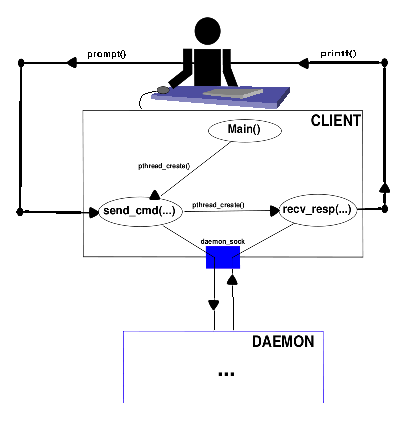
\includegraphics[scale=0.8]{archi_client.eps}
\end{figure}
\end{center}


\end{frame}

\begin{frame}
    \textbf{Le démon}
    
    \begin{itemize}
        \item Exécution en arrière-plan
        \item Gestion de toutes les requêtes (clients et démons)
        \item Vision globale : liste de clients et démons connus
        \item Utilisation des pools de threads :
            \begin{itemize}
                \item N threads créés au démarrage du démon
                \item Dorment en attendant des tâches
                \item Tâches "rapides" et tâches "lentes"
            \end{itemize}
     \end{itemize}
\begin{center}
\begin{figure}[htbp]
    \centering
    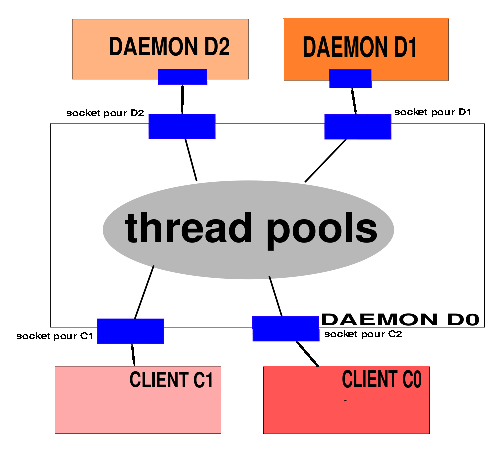
\includegraphics[scale=0.5]{archi_daemon.eps}
\end{figure}
\end{center}

\end{frame}

\begin{frame}
    \section{Gestion des threads}

    \textbf{Gestion des threads}

    Structure : 1 thread principal et 4 pools.
\begin{center}
\begin{figure}[htbp]
    \centering
    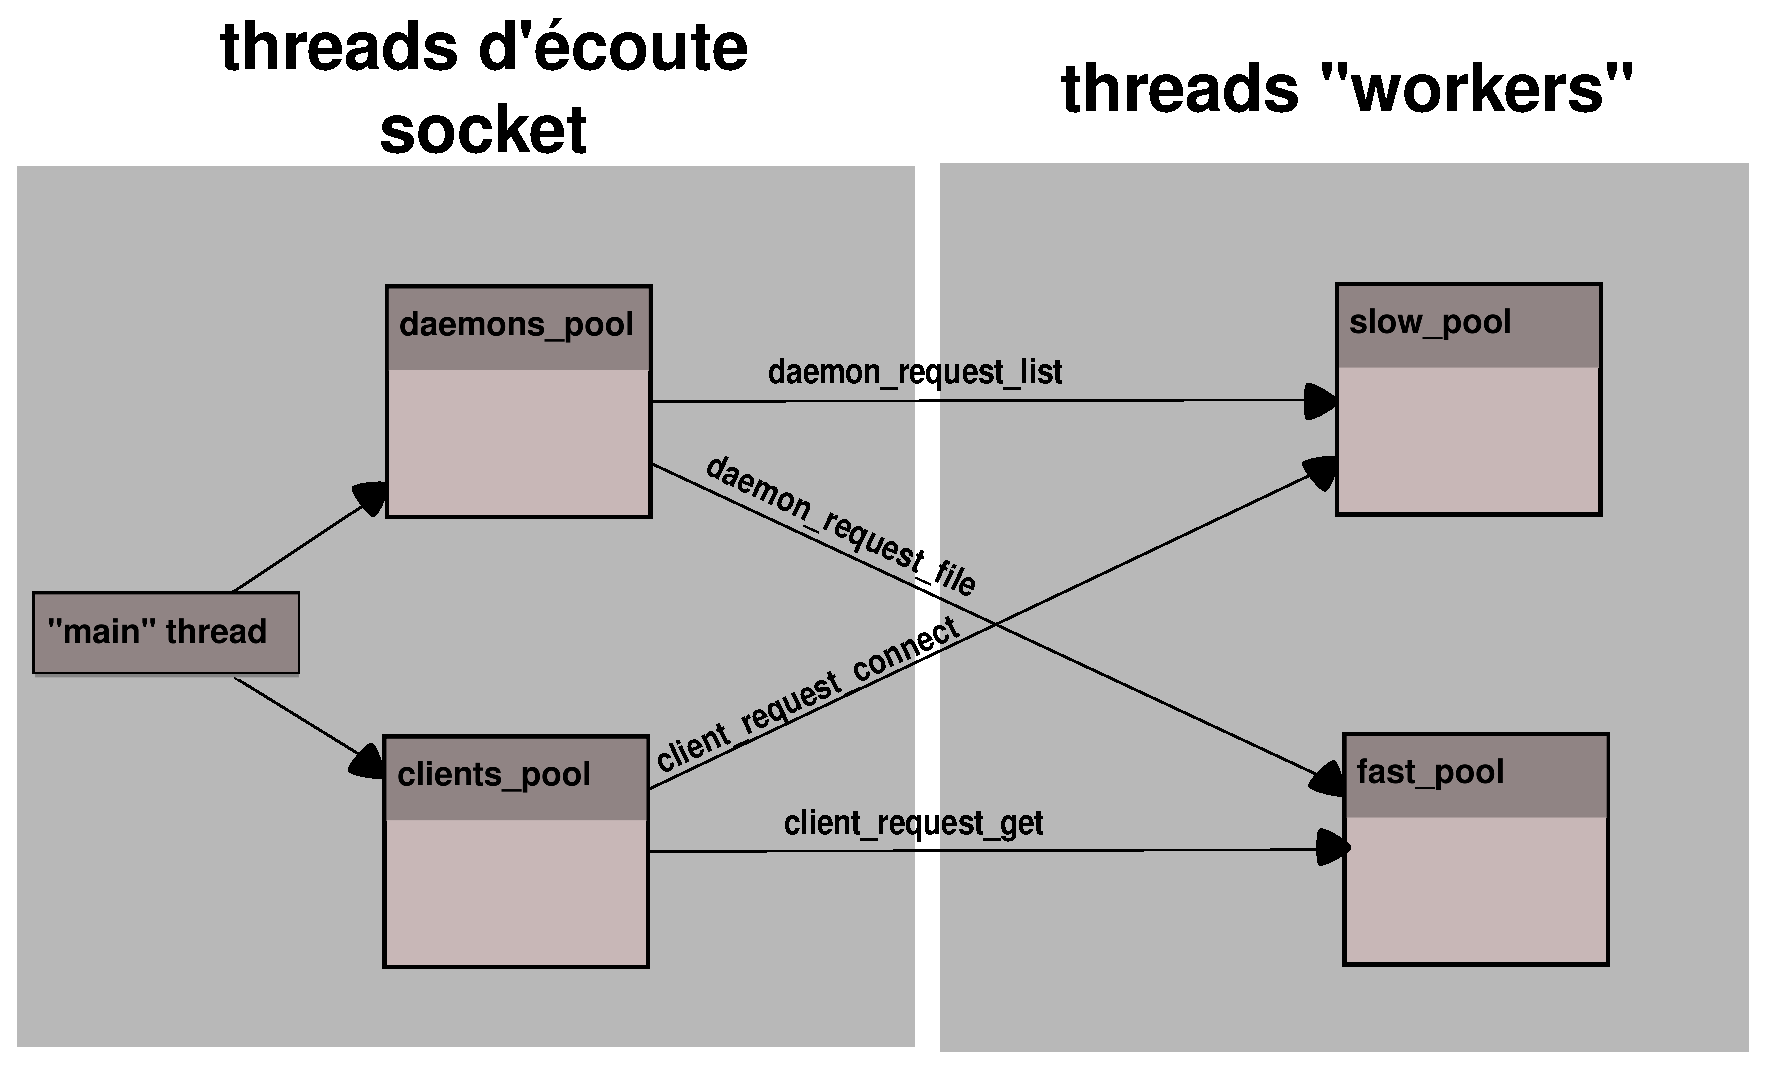
\includegraphics[scale=0.4]{pools_interacting.eps}
\end{figure}
\end{center}

\end{frame}

\begin{frame}
    \begin{itemize}
        \item 2 pools pour les clients et les démons
        \item 2 pools pour les requêtes rapides et lentes
    \end{itemize}
\begin{center}
\begin{figure}[htbp]
    \centering
    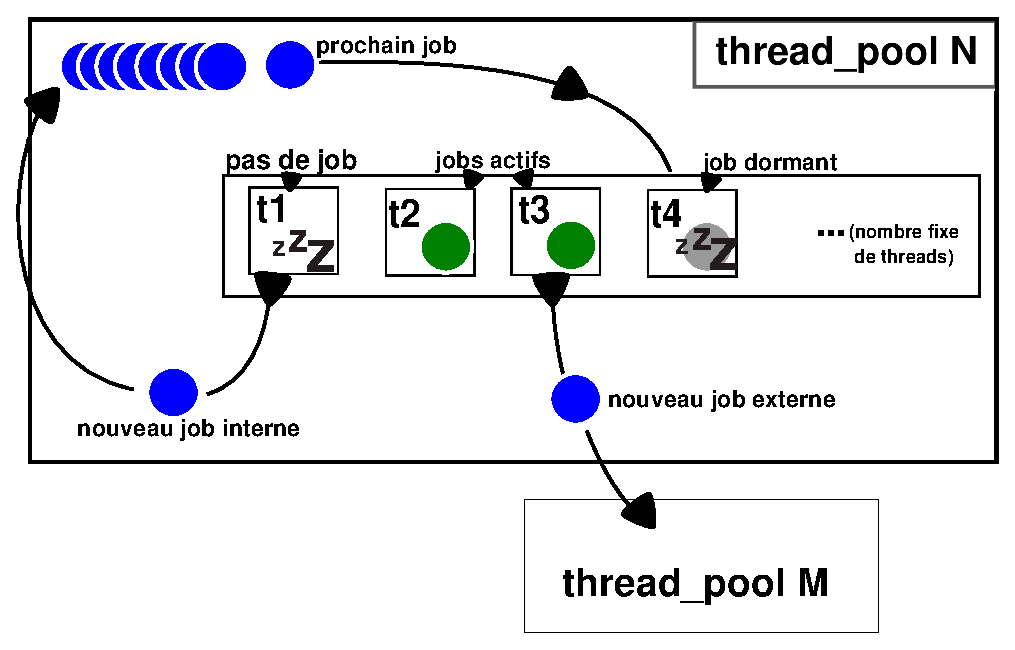
\includegraphics[scale=0.6]{thread_pool.eps}
\end{figure}
\end{center}

\end{frame}

\begin{frame}
    \section{Requêtes}

    \textbf{Requêtes implémentées}
    \begin{itemize}
        \item Commandes de protocole :
            \begin{itemize}
                \item list
                \item file fichier hash taille ip:port
                \item get hash debut fin
                \item ready hash délai ip port protocole début fin
                \item neighbourhood
                \item neighbour ip:port
                \item error
            \end{itemize}
        \item Commandes utilisateur :
            \begin{itemize}
                \item set
                \item help
                \item list
                \item get hash
                \item info
                \item download
                \item upload
                \item connect ip:port
                \item raw ip:port cmd
            \end{itemize}
    \end{itemize}
\end{frame}

\begin{frame}
    \textbf{Requêtes non implémentées}
    \begin{itemize}
        \item traffic
        \item checksum hash taille-bloc début fin checksum
        \item redirect hash ip:port
    \end{itemize}
\end{frame}

\begin{frame}
    \section{Transfert bloc par bloc}

    \textbf{Transfert bloc par bloc}
\end{frame}

\end{document}
